% % -*- coding:utf-8 -*-
\documentclass[aspectratio=169,10pt]{beamer}
\nonstopmode

\usepackage{appendixnumberbeamer}
\usepackage{graphicx}
\usepackage{url}
\usepackage{pdfpages}
% color palette
\definecolor{tu01}{HTML}{84B818}
\definecolor{tu02}{HTML}{D18B12}
\definecolor{tu03}{HTML}{1BB5B5}
\definecolor{tu04}{HTML}{F85A3E}
\definecolor{tu05}{HTML}{4B6CFC}
\definecolor{tu06}{HTML}{E3B505}
\definecolor{tu07}{HTML}{AF331D}
\definecolor{tu08}{HTML}{000000}
\definecolor{tu09}{HTML}{AAAAAA}
\definecolor{tu10}{HTML}{444444}
\definecolor{tu11}{HTML}{84B818}

% mixed and light colors
\colorlet{tu01light}{tu01!33}
\colorlet{tu02light}{tu02!33}
\colorlet{tu03light}{tu03!33}
\colorlet{tu04light}{tu04!33}
\colorlet{tu05light}{tu05!33}
\colorlet{tu06light}{tu06!33}
\colorlet{tu07light}{tu07!33}
\colorlet{tu08light}{tu08!33}
\colorlet{tu09light}{tu09!33}
\colorlet{tu10light}{tu10!33}
\colorlet{tu11light}{tu11!33}

\colorlet{tu01midlight}{tu01!50}
\colorlet{tu02midlight}{tu02!50}
\colorlet{tu03midlight}{tu03!50}
\colorlet{tu04midlight}{tu04!50}
\colorlet{tu05midlight}{tu05!50}
\colorlet{tu06midlight}{tu06!50}
\colorlet{tu07midlight}{tu07!50}
\colorlet{tu08midlight}{tu08!50}
\colorlet{tu09midlight}{tu09!50}
\colorlet{tu10midlight}{tu10!50}
\colorlet{tu11midlight}{tu11!50}

\colorlet{tu01dark}{tu01!80!black}
\colorlet{tu02dark}{tu02!80!black}
\colorlet{tu03dark}{tu03!80!black}
\colorlet{tu04dark}{tu04!80!black}
\colorlet{tu05dark}{tu05!80!black}
\colorlet{tu06dark}{tu06!80!black}
\colorlet{tu07dark}{tu07!80!black}
\colorlet{tu08dark}{tu08!80!black}
\colorlet{tu09dark}{tu09!80!black}
\colorlet{tu10dark}{tu10!80!black}
\colorlet{tu11dark}{tu11!80!black}

\colorlet{lightgray}{gray!25}
\colorlet{midlightgray}{gray!50}
\colorlet{anthracite}{black!85}

% aliases
\colorlet{tudo}{tu01}
\colorlet{tuorange}{tu02}
\colorlet{tudolight}{tu01light}

% \usepackage{beamerthememetropolis}
\usetheme[progressbar=frametitle,noslidenumbers]{metropolis}
\newcommand{\themename}{\textbf{\textsc{metropolis}}\xspace}


\usepackage{xcolor}



\title{Pr\"asentation Bachelor Arbeit:\\
 Simulation von Online Scheduling-Algorithmen f\"ur parallele Systeme}
% \subtitle{Learning to Identify Similarities between Mathematical Expressions}
\author{Hendrik Rassmann}

\institute{TU Dortmund University - Department of Computer Science}
\titlegraphic{\hfill
\includegraphics[height=8mm]{tu-do-logo.pdf}}

\date{November 02, 2020}

\begin{document}


\maketitle
\Large

\begin{frame}{\"Ubersicht}
\tableofcontents
\end{frame}


\begin{frame}[fragile]{Startpunkt}

\begin{columns}
	\begin{column}{0.57\paperwidth}
		\vspace{0.5pt}
		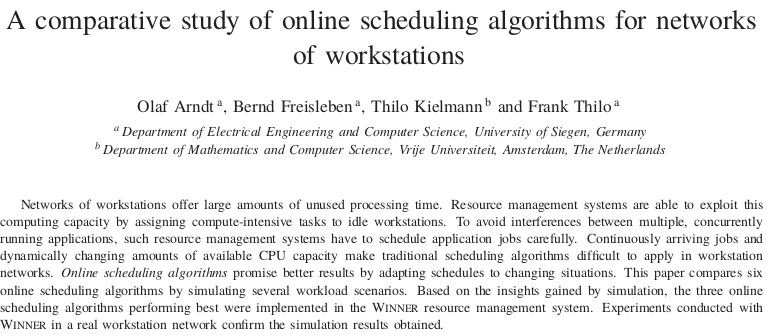
\includegraphics[width=\linewidth, clip]{images/Arndt}
	\end{column}
	\begin{column}[c]{0.43\paperwidth}
		\begin{itemize}
			\item \alert{Network}
			\item \alert{Online}
			\item \alert{Experiments} ... \alert{confirm}
		\end{itemize}
	\end{column}
\end{columns}
\end{frame}
\section{Problemstellung}


\begin{frame}[t,fragile]{Problemstellung}
Ausgehend von:

\begin{itemize}[<+->]
	\item Rechner/\emph{Nodes} unterschiedlicher \emph{Geschwindigkeiten} bilden zusammen ein (Rechen)\emph{Cluster} 
	\item Auftr\"age/\emph{Jobs} kommen im laufenden Betrieb rein (\emph{online})
	\item Auftr\"age unterscheiden sich bez. \emph{Bearbeitungszeit}, \emph{Anzahl} an ben\"otigten Knoten und \emph{Ankunftszeitpunkt}
	\item Auftr\"age sollen auf eine 'geeignete' Art und Weise bearbeitet werden
\end{itemize}
\end{frame}


\begin{frame}[t,fragile]{Zielfunktionen \footnote{Kriterien von Arndt. et al.}}
\begin{itemize}[<+->]
	\item \emph{makespan} ''Zeit bis Feierabend''
	\item \emph{average flow time} ''Supermarkt - Nur der Apfel? Gehen Sie doch gerne vor''
	\item \emph{average waiting time} 	
	\item \emph{maximum waiting time} ''Restaurant - Wenn ein Tisch nicht bedient wird, kommen G\"aste nicht mehr wieder''
\end{itemize}
\end{frame}

\begin{frame}[t, fragile]{Scheduling-Algorithmen (Referentiell Transparent)\footnote{Auswahl von Arndt. et al.}} 
$Scheduling$-$Algorithmus : Warteliste \rightarrow Auftrag$\\
\pause

\begin{itemize}[<+->]
	\item First in First out (\emph{FiFo})
	\item Shortest Processing Time first (\emph{SPT})
	\item Greates Processing Time first (\emph{GPT})
\end{itemize}
\end{frame}



%
\includegraphics[page=1, scale=0.4]{SchedulingBeispiel.pdf}
\setbeamercolor{background canvas}{bg=}

\includepdf[pages=2-]{SchedulingBeispiel.pdf}

\begin{frame}[t, fragile]{Scheduling-Algorithmen (Referentiell Intransparent)}
\begin{itemize}[<+->]
	\item Random
	\item \alert{First Fit} (W\"ahle den am l\"angsten wartende Auftrag, der sofort gestartet werden kann)
	\item \alert{Backfilling} (W\"ahle einen startbaren Auftrag, der wenn er jetzt gestartet wird, terminiert bevor der am l\"angsten wartende Auftrag starten wird)
\end{itemize}
\end{frame}

\begin{frame}[t, fragile]{Beispiel Backfilling}
\end{frame}
\setbeamercolor{background canvas}{bg=}
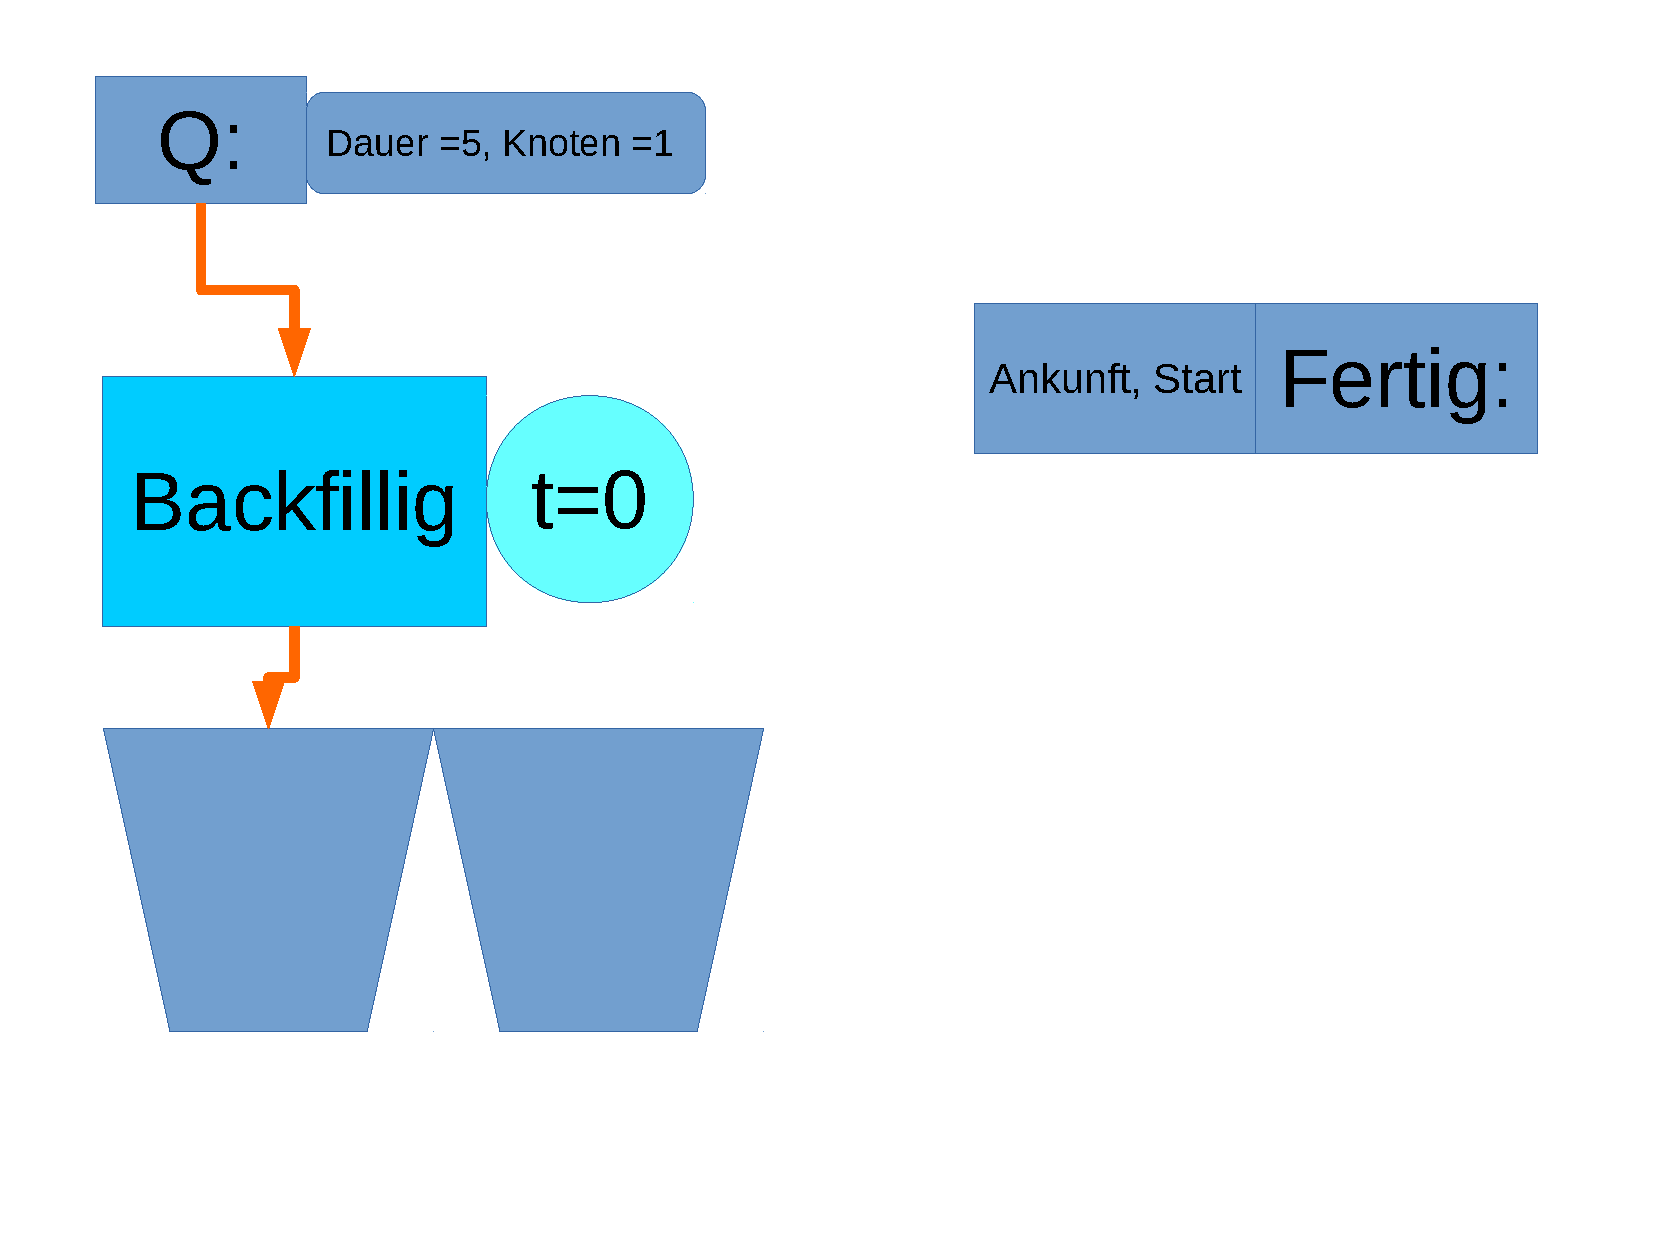
\includepdf[pages=-]{SchedulingBeispiel2.pdf}


\section{Simulationsaufbau}

\begin{frame}[t, fragile]{Simulations Paradigma\footnote{Matloff, Norm: Introduction to discrete-event simulati-
		on and the simpy language. In: Davis, CA. Dept of Com-
		puter Science. University of California at Davis. Retrieved on
		August 2 (2008), Nr. 2009, S. 1–33}}
	\begin{itemize}
		\item Aktivit\"atsorientiert (Wettersystem, Physik Simulation in Videospielen)
		\item \alert{Ereignisorientiert} (Fahrplan)
		\item Prozessorientiert (Parallele Programmierung)
	\end{itemize}
\end{frame}

\begin{frame}[t, fragile]{Simulation und Auswertung}
	\begin{itemize}
		\item Arndt et al. \alert{designen Experimente}, um unterschiedliches Verhalten der Algorithmen zu demonstrieren
		\item Variieren einen Parameter und vergleichen gew\"ahlte Zielfunktionen
	\end{itemize}
\end{frame}

\begin{frame}[fragile]{Beispiel}

\begin{columns}
	\begin{column}{0.57\paperwidth}
		\vspace{0.5pt}
		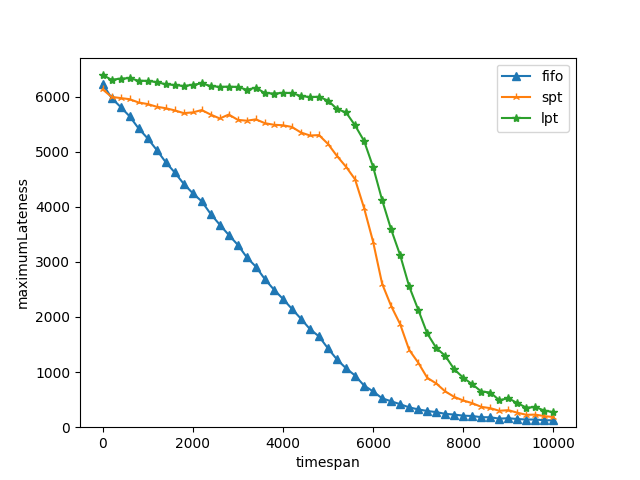
\includegraphics[width=\linewidth, clip]{images/Figure_2_2}
	\end{column}
	\begin{column}[c]{0.43\paperwidth}
		\begin{itemize}
			\item timespan - Sp\"atester Ankunftszeitpunkt wird variiert
			\item Latenz am besten bei FiFo
			\item An beiden Extremen \"ahnliches Verhalten
		\end{itemize}
	\end{column}
\end{columns}
\end{frame}

%-------------------------------------------
\section{Outlook}
\begin{frame}{Outlook}
\Large
The font size should be as large as possible
\begin{itemize}
\item \textit{Never smaller than the age of the oldest audience member}
\item Don't vary sizes to much, never within a slide
\item Stick to one font
\item Don't overuse formatting like bold, italics, alert, etc.
\end{itemize}
But you knew all that already...
\end{frame}

\begin{frame}[t,fragile]{Querying Data used to be simple...}
\begin{itemize}
	\item Tutorial for Beamer \url{https://www.overleaf.com/learn/latex/Beamer_Presentations:_A_Tutorial_for_Beginners_(Part_1)%E2%80%94Getting_Started}
		\item Quelle Template: \url{https://github.com/matze/mtheme}
		\item Quelle Bild: \url{https://unsplash.com/photos/52gEprMkp7M}
	\end{itemize}
\end{frame}

\begin{frame}[fragile]{How about a very large image?}

\begin{columns}
	\begin{column}{0.57\paperwidth}
		\vspace{0.5pt}
		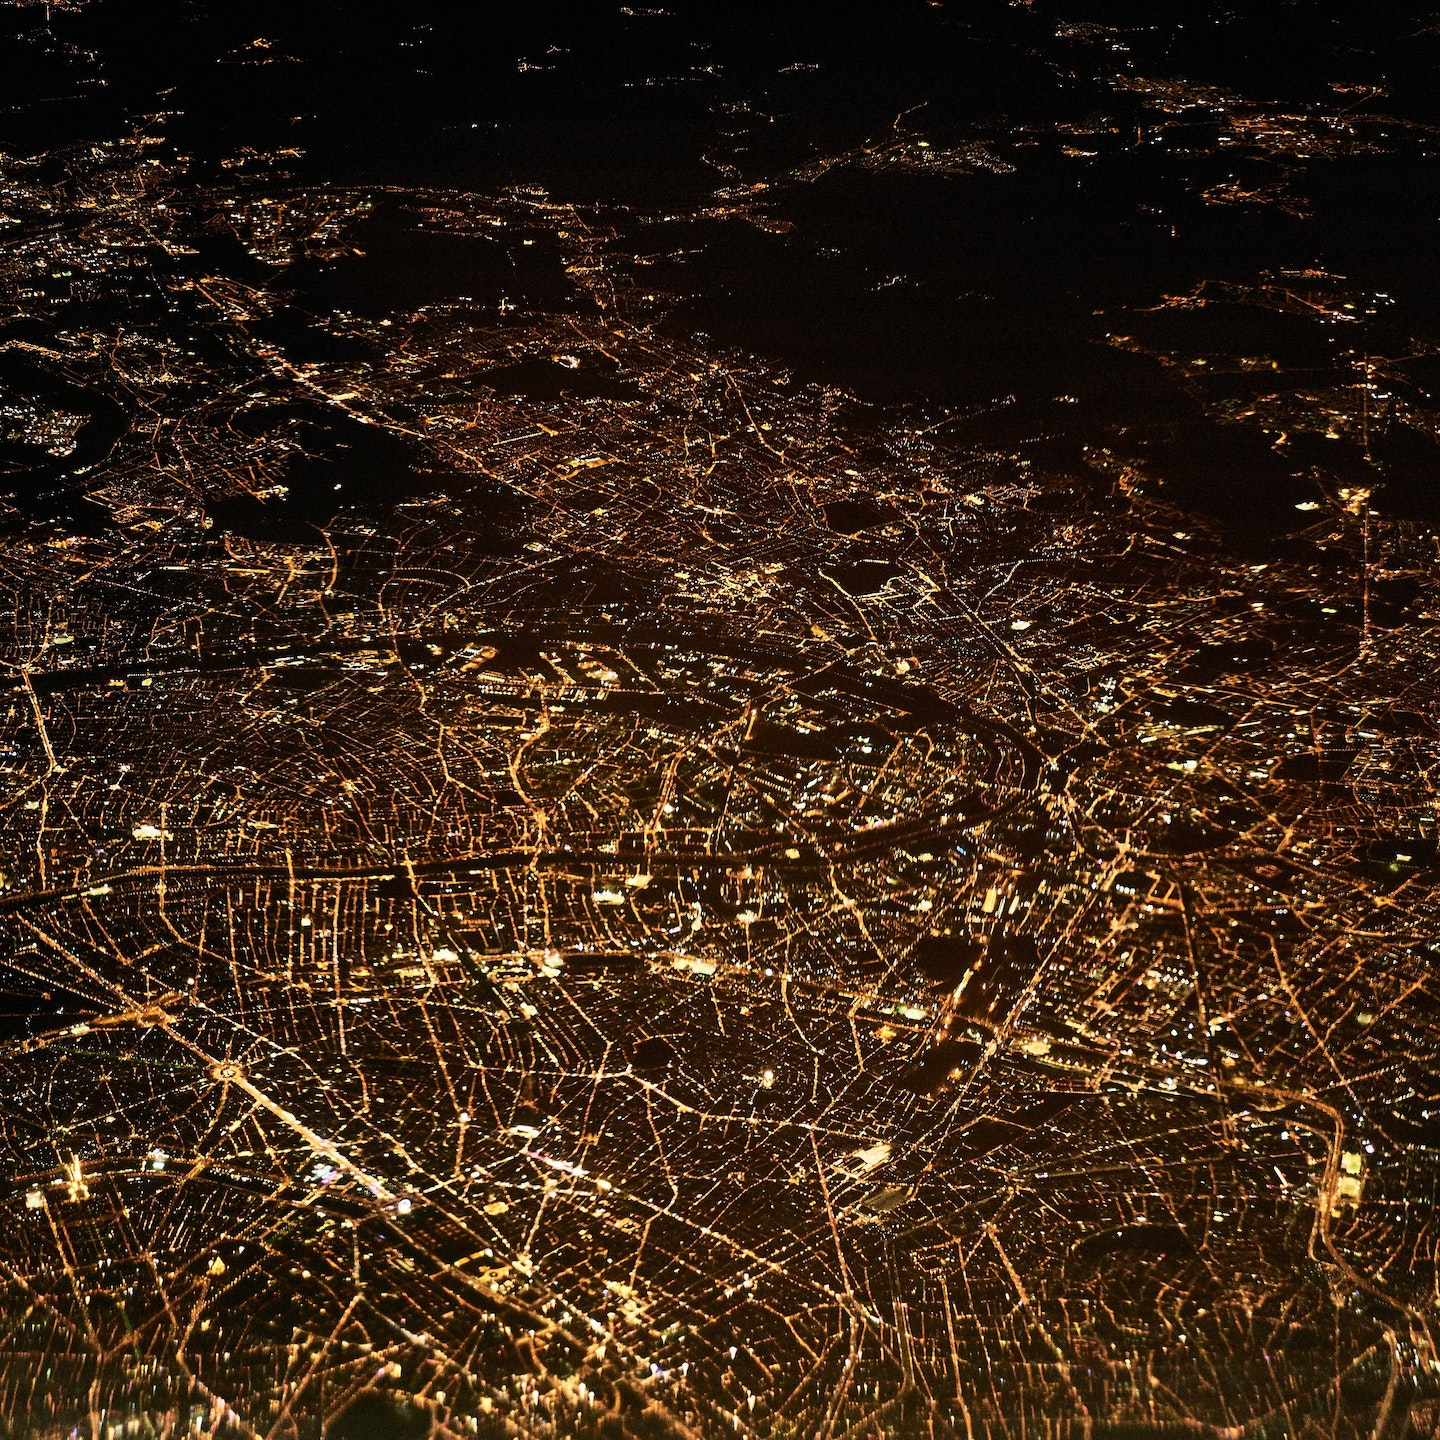
\includegraphics[width=\linewidth, clip]{images/city}
	\end{column}
	\begin{column}[c]{0.43\paperwidth}
		\begin{itemize}
			\item Itemize Environments are important
			\item We can \alert{highlight} words
			\pause
			\item We can add animations.\\(please don't over-do it)
		\end{itemize}
	\end{column}
\end{columns}
\end{frame}

\begin{frame}[t,standout]
\Large
Clever Last Words to Stimulate Discussion
\end{frame}

\end{document}
